\documentclass[11pt]{article}
\usepackage{amsmath}
\usepackage{graphicx}
\usepackage{hyperref}
\usepackage[utf8]{inputenc}
\usepackage[spanish]{babel}
\usepackage[margin=2.5cm]{geometry}
\usepackage{amsfonts}
\usepackage{listings}
\usepackage{textcomp}
\usepackage{float}
\usepackage[T1]{fontenc}

\title{Big Analysis con Spark.}
\author{Néstor Rodríguez Vico - \href{mailto:nrv23@correo.ugr.es}{nrv23@correo.ugr.es}}
\date{\today}

\begin{document}
\maketitle

\section{Introducción.}

En esta práctica hemos probado diferentes algoritmos de preprocesamiento y diferentes clasificadores de \textit{Spark} (\href{https://spark.apache.org/}{https://spark.apache.org/}) para abordar un problema de Big Data. Dichas prácticas se han ejecutado en un clúster proporcionado por la universidad con \textit{216} núcleos y \textit{696.0 GB} de memoria RAM.

\section{Metodología de trabajo.}

Para abordar la práctica, se ha usado la máquina virtual proporcionada por el profesorado. En dicha máquina, he desarrollado el código, compilado el mismo y ejecutado con los conjuntos de datos reducidos hasta asegurarme de que los algoritmos no producían ningún error descontrolado. Una vez tenía un código completamente ejecutable, lo he compilado, subido al \textit{clúster} y ejecutado, guardando los resultados en un fichero de salida para poder revisarlos posteriormente. \\

Para comparar los algoritmos de clasificación y ver el rendimiento de los algoritmos de preprocesamiento aplicados he usado el valor de la métrica \textit{AUC} (\textit{área under the curve}). La representación de dicha métrica la podemos ver en la siguiente figura:

\begin{figure}[H]
	\centering
	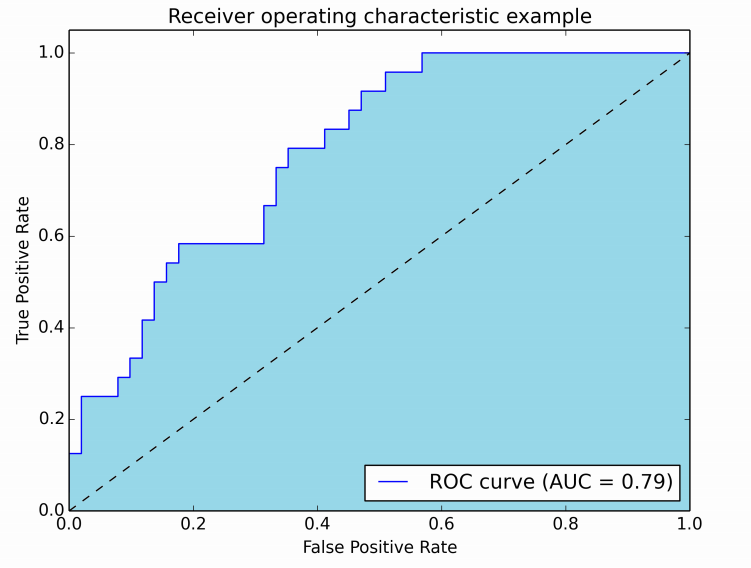
\includegraphics[width=0.5\linewidth]{images/AUC.png}
\end{figure}

Dicha métrica representa el área bajo la curva que se obtiene al representar el ratio de verdaderos positivos frente al ratio de falsos positivos. A mayor valor de \textit{AUC}, mejor es el modelo aprendido.

\section{Análisis inicial.}

Lo primero que he hecho es estudiar el balanceo y si hay valores perdidos en el conjunto de datos. En el conjunto de datos disponible en el clúster contamos con \textit{900000} instancias asociada a la clase \textit{0.0} y \textit{100000} instancias asociada a la clase \textit{1.0}, lo cual nos indica que nos enfrentamos a un problema bastante desbalanceado, con un ratio de desbalanceo \textit{IR = 9.0}. Con respecto a los valores perdidos se ha comprobado que estos no existen, así que no tenemos que lidiar con algoritmos de preprocesamiento que apliquen imputación de valores perdidos.

\section{Preprocesamiento.}

En esta sección voy a comentar los distintos algoritmos aplicados de preprocesamiento. Cuando hable de los parámetros de los algoritmos, voy a marcar con un asterísco (\textit{*}) los parámetros cuyos valores han sido obtenidos de forma empírica realizando varias pruebas, debido a la dificultad de hacer optimización de parámetros en un problema de estas dimensiones.

\subsection{Desbalanceo.}

Para corregir el desbalanceo se han implementado algoritmos dos algoritmos, \textit{RandomOversampling} y \textit{RandomUndersampling}. Las implementaciones propuestas se basan en las realizadas por \textit{Sara Del Río García}, las cuales podemos encontrar en su \href{https://github.com/saradelrio/Imb-sampling-ROS_and_RUS}{GitHub}.

\subsection{Limpieza de ruido.}

Para limpiar el ruido se han usado los siguientes algoritmos:

\begin{itemize}
	\item \textit{HME\_BD}: implementado por \textit{Diego García}. Dicha implementación se encuentra disponible en su repositorio \href{https://github.com/djgarcia/NoiseFramework}{NoiseFramework} en GitHub. Dicho algoritmo se ha ejecutado con los parámetros:
	
	\begin{itemize}
		\item \textit{data}: Conjunto de datos a procesar.
		\item \textit{(*) nTrees = 100}: Número de árboles a crear.
		\item \textit{(*) k = 4}: Número de particiones.
		\item \textit{(*) maxDepth = 10}: Profundidad máxima de los árboles.
		\item \textit{seed = 0}: Semilla para inicializar el generador de números aleatorios.
	\end{itemize}

	\item \textit{HTE\_BD}: implementado por \textit{Diego García}. Dicha implementación se encuentra disponible en su repositorio \href{https://github.com/djgarcia/NoiseFramework}{NoiseFramework} en GitHub. Dicho algoritmo se ha ejecutado con los parámetros:
	
	\begin{itemize}
		\item \textit{data}: Conjunto de datos a procesar.
		\item \textit{(*) nTrees = 100}: Número de árboles a crear.
		\item \textit{(*) partitions = 4}: Número de particiones.
		\item \textit{(*) vote = 0}: Estragia en el proceso de votación. Un cero indica \textit{mayoría}.
		\item \textit{(*) partitions = 4}: Número de vecinos.
		\item \textit{(*) maxDepth = 10}: Profundidad máxima de los árboles.
		\item \textit{seed = 0}: Semilla para inicializar el generador de números aleatorios.
	\end{itemize}
	
	\item \textit{ENN\_BD}: implementado por \textit{Diego García}. Dicha implementación se encuentra disponible en su repositorio \href{https://github.com/djgarcia/NoiseFramework}{NoiseFramework} en GitHub. Dicho algoritmo se ha ejecutado con los parámetros:
	
	\begin{itemize}
		\item \textit{data}: Conjunto de datos a procesar.
		\item \textit{(*) k = 4}: Número de vecinos.
	\end{itemize}
	
	\item \textit{NCNEdit\_BD}: implementado por \textit{Diego García}. Dicha implementación se encuentra disponible en su repositorio \href{https://github.com/djgarcia/SmartFiltering}{SmartFiltering} en GitHub. Dicho algoritmo se ha ejecutado con los parámetros:
	
	\begin{itemize}
		\item \textit{data}: Conjunto de datos a procesar.
		\item \textit{(*) k = 4}: Número de vecinos.
	\end{itemize}
	
\end{itemize}

También he probado \textit{RNG\_BD}, implementado por \textit{Diego García}, disponible en su repositorio \href{https://github.com/djgarcia/SmartFiltering}{SmartFiltering} en GitHub. Dicho algoritmo lanza una excepción \textit{ java.lang.OutOfMemoryError: Java heap space}, la cual no he podido solucionar y, por lo tanto, no he podido ejecutarlo.

\subsection{Discretización.}

Para discretizar los datos se ha usado el algoritmo \textit{EqualWidthDiscretizer} implementado por \textit{Diego García} el cual se encuentra disponible en su repositorio \href{https://github.com/djgarcia/Equal-Width-Discretizer}{Equal-Width-Discretizer} en GitHub. Dicho algoritmo se ha ejecutado con los parámetros:

\begin{itemize}
	\item \textit{data}: Conjunto de datos a procesar.
	\item \textit{(*) nBins = 25}: Número de \textit{bins} a crear..
\end{itemize}

\subsection{Selección de características.}

Nos encontramos ante un dataset de un millón de instancias y dieciocho características. Como podemos ver, el cuello de botella del problema es el número de instancias, no el número de características. Aplicar un algoritmo de selección de características para un millón de instancias teniendo sólo dieciocho características no tiene mucho sentido, ya que vamos a tener que invertir mucho tiempo de cómputo en reducir la dimensionalidad, a pesar de que esta ya es pequeña. \\

Para probar lo comentado anteriormente, se ha usado un algoritmo de \textit{PCA} implementado en la librería \href{https://spark.apache.org/docs/2.2.0/api/scala/index.html#org.apache.spark.ml.feature.PCA}{mllib}. Este algotimo necesita ningún parámetro para funcionar, sólo el conjunto de datos a procesar y el número de componente principales a elegir, en mi caso he elegido \textit{5}, para reducir la dimensionalidad a un \textit{30\%} de la original.

\subsection{Selección de instancias.}

Para la selección de instancias se han usado los siguientes algoritmos:

\begin{itemize}
	\item \textit{FCNN\_MR}: implementado por \textit{Diego García}. Dicha implementación se encuentra disponible en su repositorio \href{https://github.com/djgarcia/SmartReduction}{SmartReduction} en GitHub. Dicho algoritmo se ha ejecutado con los parámetros:
	
	\begin{itemize}
		\item \textit{data}: Conjunto de datos a procesar.
		\item \textit{(*) k = 3}: Número de vecinos.
	\end{itemize}

	\item \textit{RMHC\_MR}: implementado por \textit{Diego García}. Dicha implementación se encuentra disponible en su repositorio \href{https://github.com/djgarcia/SmartReduction}{SmartReduction} en GitHub. Dicho algoritmo se ha ejecutado con los parámetros:
	
	\begin{itemize}
		\item \textit{data}: Conjunto de datos a procesar.
		\item \textit{(*) p = 0.1}: Porcentaje de instancias.
		\item \textit{(*) it = 100}: Número de iteraciones.
		\item \textit{(*) k = 3}: Número de vecinos.
		\item \textit{seed = 0}: Semilla para inicializar el generador de números aleatorios.
	\end{itemize}
\end{itemize}

También he intentado probar el algoritmo \textit{SSMASFLSDE\_MR}, implementado por \textit{Diego García}, disponible en su repositorio \href{https://github.com/djgarcia/SmartReduction}{SmartReduction} en GitHub. El prblema de dicho algoritmo es que se trata de un algoritmo evolutivo y consume mucho tiempo, así que he decidido no ejecutarlo, ya que tenemos otros algoritmos de selección de instancias que funcionan bastante bien y son más rápidos.

\section{Clasificadores.}

En esta sección voy a comentar los clasificadores usados en esta práctica. Cuando hable de los parámetros de los algoritmos, voy a marcar con un asterísco (\textit{*}) los parámetros cuyos valores han sido obtenidos de forma empírica realizando varias pruebas, debido a la dificultad de hacer optimización de parámetros en un problema de estas dimensiones.

\subsection{Random Forest.}

El primer clasificador probado es un \textit{Random Forest} estándar. El algoritmo usado ha sido \href{https://spark.apache.org/docs/2.2.0/api/scala/index.html#org.apache.spark.mllib.tree.RandomForest}{\textit{RandomForest}}, disponible en la biblioteca \textit{mllib}. El código usado para entrenar dicho clasificador es el siguiente:

\begin{lstlisting}[frame=single, language=scala, xleftmargin=.25in, basicstyle=\small, upquote=true, breaklines = true]
RandomForest.trainClassifier(train, numClasses = 2, 
	categoricalFeaturesInfo = Map[Int, Int](), numTrees = 80, 
	featureSubsetStrategy = "auto", impurity = "gini", maxDepth = 8, 
	maxBins = 32, seed = 0)
\end{lstlisting}

Explicación de los parámetros:

\begin{itemize}
	\item \textit{train}: Conjunto de entrenamiento.
	\item \textit{numClasses}: Número de clases de nuestro problema.
	\item \textit{categoricalFeaturesInfo}: Información sobre las variables categóricas. Nuestro problema no tiene variables categóricas, por eso pasamos un \textit{Map} vacío.
	\item \textit{(*) numTrees}: Número de árboles a generar.
	\item \textit{featureSubsetStrategy}: Número de características a considerar para las divisiones en cada nodo. Si se usa \textit{auto} el algoritmo determinará el mejor valor basándose en el valor de \textit{numTrees}.
	\item \textit{impurity}: Criterio utilizado para el cálculo de la ganancia de información. Se ha usado \textit{gini} ya que es el recomendado por la documentación.
	\item \textit{(*) maxDepth}: Profundida máxima del árbol.
	\item \textit{(*) maxBins}: Número máximo de \textit{bins} utilizadas para el particionamiento.
	\item \textit{seed}: Semilla para inicializar el generador de números aleatorios.
\end{itemize}

\subsection{SVMwithSGD.}

A continuación se ha usado una \textit{máquina de soporte vectorial} (\textit{Support Vector Machine - SVM}) que hace uso del \textit{gradiente descendente estocástico} (\textit{Stochastic Gradient Descent - SGD}). El algoritmo usado ha sido \href{https://spark.apache.org/docs/2.2.0/api/scala/index.html#org.apache.spark.mllib.classification.SVMWithSGD}{\textit{SVMWithSGD}}, disponible en la biblioteca \textit{mllib}. El código usado para entrenar dicho clasificador es el siguiente:

\begin{lstlisting}[frame=single, language=scala, xleftmargin=.25in, basicstyle=\small, upquote=true, breaklines = true]
SVMWithSGD.train(train, numIterations = 100)
\end{lstlisting}

Explicación de los parámetros:

\begin{itemize}
	\item \textit{train}: Conjunto de entrenamiento.
	\item \textit{(*) numIterations}: Número de iteraciones.
\end{itemize}

\subsection{PCARD.}

El algoritmo \textit{PCARD} es un ensemble. El algoritmo usado ha sido \href{https://github.com/djgarcia/PCARD}{\textit{PCARD}}, disponible en el repositorio de \textit{GitHub} de \textit{Diego García}. El código usado para entrenar dicho clasificador es el siguiente:

\begin{lstlisting}[frame=single, language=scala, xleftmargin=.25in, basicstyle=\small, upquote=true, breaklines = true]
PCARD.train(train, nTrees = 100, cuts = 5)
\end{lstlisting}

Explicación de los parámetros:

\begin{itemize}
	\item \textit{train}: Conjunto de entrenamiento.
	\item \textit{(*) numTrees}: Número de árboles a generar.
	\item \textit{(*) cuts}: Número de umbrales por característica.
\end{itemize}

\subsection{Decision Tree.}

Este algoritmos es un árbol de decicisón clásico. El algoritmo usado ha sido \href{https://spark.apache.org/docs/2.2.0/api/scala/index.html#org.apache.spark.mllib.tree.DecisionTree}{\textit{DecisionTree}}, disponible en la biblioteca \textit{mllib}. El código usado para entrenar dicho clasificador es el siguiente:

\begin{lstlisting}[frame=single, language=scala, xleftmargin=.25in, basicstyle=\small, upquote=true, breaklines = true]
DecisionTree.trainClassifier(train, numClasses = 2, 
	categoricalFeaturesInfo = Map[Int, Int](), impurity = "gini", 
	maxDepth = 8, maxBins = 32)
\end{lstlisting}

Explicación de los parámetros:

\begin{itemize}
	\item \textit{train}: Conjunto de entrenamiento.
	\item \textit{numClasses}: Número de clases de nuestro problema.
	\item \textit{categoricalFeaturesInfo}: Información sobre las variables categóricas. Nuestro problema no tiene variables categóricas, por eso pasamos un \textit{Map} vacío.
	\item \textit{impurity}: Criterio utilizado para el cálculo de la ganancia de información. Se ha usado \textit{gini} ya que es el recomendado por la documentación.
	\item \textit{(*) maxDepth}: Profundida máxima del árbol.
	\item \textit{(*) maxBins}: Número máximo de \textit{bins} utilizadas para el particionamiento.
\end{itemize}

\subsection{GradientBoostedTrees.}

Este algoritmo se basa en el algoritmo \textit{Stochastic Gradient Boosting} propuesto por \textit{J.H. Friedman} en 1999. Dicho algoritmo aprende conjuntos de árboles minimizando la funcion de pérdida. El algoritmo usado ha sido \href{https://spark.apache.org/docs/2.2.0/api/scala/index.html#org.apache.spark.mllib.tree.GradientBoostedTrees}{\textit{GradientBoostedTrees}} disponible en la biblioteca \textit{mllib}. El código usado para entrenar dicho clasificador es el siguiente:

\begin{lstlisting}[frame=single, language=scala, xleftmargin=.25in, basicstyle=\small, upquote=true, breaklines = true]
val boostingStrategy = BoostingStrategy.defaultParams("Classification")
boostingStrategy.numIterations = 100
boostingStrategy.treeStrategy.numClasses = 2
boostingStrategy.treeStrategy.maxDepth = 5
boostingStrategy.treeStrategy.categoricalFeaturesInfo = Map[Int, Int]()

GradientBoostedTrees.train(train, boostingStrategy)
\end{lstlisting}

Explicación de los parámetros:

\begin{itemize}
	\item \textit{(*) boostingStrategy.numIterations}: Número de iteraciones.
	\item \textit{boostingStrategy.treeStrategy.numClasses}: Número de clases de nuestro problema.
	\item \textit{(*) boostingStrategy.treeStrategy.maxDepth}: Profundida máxima del árbol.
	\item \textit{boostingStrategy.treeStrategy.categoricalFeaturesInfo}: Información sobre las variables categóricas. Nuestro problema no tiene variables categóricas, por eso pasamos un \textit{Map} vacío.
	\item \textit{train}: conjunto de entrenamiento.
\end{itemize}

\section{Experimentos.}

En esta sección voy a detallar los experimentos realizados. Los parámetros usados en los experimentos han sido los indicados en las secciones anteriores si no se indica lo contrario.

\subsection{Experimentos básicos.}

Lo primero que he hecho ha sido aplicar todos los clasificadores a todas las técnicas de preprocesamiento de forma independiente, es decir, sin combinaciones entre ellos. Tras asplicar una técnica de preprocesamiento que modifica el ratio de desbalanceo (como puede ser \textit{RandomOversampling}, \textit{RandomUndersampling} o técnicas de selección de instancias), se ha estudiado como de balanceado ha quedado el nuevo conjunto. Los valores de la métrica \textit{auc} obtenidos son los siguientes:

\begin{table}[H]
	\centering
	\resizebox{\linewidth}{!}{%
	\tabcolsep=2pt
	\begin{tabular}{rccccccccccc}
		&  & \multicolumn{2}{c}{\textbf{Sampling}} & \multicolumn{4}{c}{\textbf{ClearNoise}} & \textbf{Discretization} & \textbf{FeatureSelection} & \multicolumn{2}{c}{\textbf{InstanceSelection}} \\
		\textbf{model} & \textbf{Original} & \textbf{Under} & \textbf{Over} & \textbf{HMEBD} & \textbf{HTEBD} & \textbf{ENNBD} & \textbf{NCNEdit} & \textbf{EWD} & \textbf{pca} & \textbf{FCNN} & \textbf{RMHC} \\ \hline
		\textbf{RF} & 0.790958 & 0.613495 & 1.000000 & 0.774220 & 0.811742 & 1.000000 & 0.805488 & 0.805488 & 0.761004 & 0.733423 & 0.796452 \\
		\textbf{SVMwithSGD} & 0.832559 & 0.833361 & 0.750734 & 0.750833 & 0.748794 & 0.750481 & 0.687568 & 0.687568 & 0.805371 & 0.815443 & 0.829624 \\
		\textbf{decisionTree} & 0.733296 & 0.610165 & 0.720580 & 0.759912 & 0.786172 & 0.738511 & 0.735937 & 0.735937 & 0.719260 & 0.700328 & 0.708826 \\
		\textbf{pcard} & 0.507549 & 0.778233 & 0.500000 & 0.515958 & 0.500424 & 0.500000 & 0.508259 & 0.508259 & 0.500000 & 0.522451 & 0.509817 \\
		\textbf{gbts} & 0.750616 & 0.621049 & 0.950001 & 0.767141 & 0.795334 & 1.000000 & 0.736438 & 0.736438 & 0.737500 & 0.720658 & 0.738069 \\ \hline
		\textbf{Media} & 0.722995 & 0.691260 & 0.784263 & 0.713613 & 0.728493 & 0.797798 & 0.694738 & 0.694738 & 0.704627 & 0.698461 & 0.716558
\end{tabular}}
\end{table}

A continuación, vamos a ver el número de instancias asociadas a cada clase tras aplicar los algoritmos de preprocesamiento:

\begin{table}[H]
	\centering
		\resizebox{0.4\linewidth}{!}{%
		\tabcolsep=2pt
			\begin{tabular}{rrrr}
			\multicolumn{1}{l}{} & \multicolumn{2}{c}{\textbf{Clase}} & \multicolumn{1}{l}{} \\
			\textbf{Dataset} & \multicolumn{1}{c}{\textbf{1.0}} & \multicolumn{1}{c}{\textbf{0.0}} & \multicolumn{1}{c}{\textbf{IR}} \\ \hline
			\textbf{Original} & 900000 & 100000 & 9,00000 \\
			\textbf{RandomUndersampling} & 99344 & 100000 & 0,99344 \\
			\textbf{RandomOversampling} & 900000 & 9017 & 99,81147 \\
			\textbf{ClearNoise.HMEBD} & 895535 & 7347 & 121,89125 \\
			\textbf{ClearNoise.HTEBD} & 898529 & 2545 & 353,05658 \\
			\textbf{ClearNoise.ENNBD} & 832977 & 7422 & 112,23080 \\
			\textbf{ClearNoise.NCNEdit} & 828959 & 31025 & 26,71907 \\
			\textbf{Discretization.EWD} & 900000 & 100000 & 9,00000 \\
			\textbf{FeatureSelection.pca} & 900000 & 100000 & 9,00000 \\
			\textbf{InstanceSelection.FCNN} & 214812 & 89106 & 2,41075 \\
			\textbf{InstanceSelection.RMHC} & 90014 & 9853 & 9,13569
	\end{tabular}}
\end{table}

Cómo podemos ver, sólo tras aplicar \textit{RandomUndersampling} nos encontramos ante un dataset balanceado. En el caso de \textit{RandomOversampling} se ha usado un ratio de \textit{1.0}, lo cual ha producido el efecto inverso al deseado, se ha reducido el número de instancias de la clase \textit{0.0} en vez de aumentarlo. También podemos ver como los algoritmos de selección de características y discretización no modifican el balanceo. \\

En cuanto a los resultados de los clasificadores, podemos ver como, en el caso de \textit{Oversampling} y de \textit{ENNBD} obtenemos un resultado de \textit{1.0} (o muy cercano a \textit{1.0}) en algunos de los clasificadores. También podemos ver que, excepto en \textit{UnderSampling}, los valores obtenidos por el algoritmo \textit{PCARD} son bastante malos. Esto no se debe a que el algoritmo sea malo, sino al desbalanceo que hay en el conjunto de datos.

\subsection{Balancear el conjunto de datos.}

Como hemos visto, balancear el conjunto de datos es algo imprescindible, ya que afecta bastante a los resultados obtenidos. Por eso, mi primera tarea para intentar combinar preprocesamientos es genera un conjunto de datos balanceado. Como hemos visto, \textit{RandomUndersampling} ya nos lo proprociona. El problema de \textit{RandomUndersampling} es que partimos de un conjunto en el que se han eliminado demasiadas instancias y sin ningún criterio, lo cual puede producir que hayamos perdido información relevante de nuestro problema. Es por ello que debemos centrarnos en generar un conjunto de datos balanceado con \textit{RandomOversampling}. Para conseguir esto he jugado con el valor del parámetro que indica el ratio de instancias a generar, los resultados son los siguientes:

\begin{table}[H]
	\centering
	\resizebox{0.8\linewidth}{!}{%
		\tabcolsep=2pt
		\begin{tabular}{rrrrllrrrrllrrrr}
		\multicolumn{1}{c}{\textbf{Ratio}} & \multicolumn{1}{c}{\textbf{1.0}} & \multicolumn{1}{c}{\textbf{0.0}} & \multicolumn{1}{c}{\textbf{IR}} &  &  & \multicolumn{1}{c}{\textbf{Ratio}} & \multicolumn{1}{c}{\textbf{1.0}} & \multicolumn{1}{c}{\textbf{0.0}} & \multicolumn{1}{c}{\textbf{IR}} &  &  & \multicolumn{1}{c}{\textbf{Ratio}} & \multicolumn{1}{c}{\textbf{1.0}} & \multicolumn{1}{c}{\textbf{0.0}} & \multicolumn{1}{c}{\textbf{IR}} \\ \hline
		\textbf{1.0} & 900000 & 9017 & 99,81147 &  &  & \textbf{35.0} & 900000 & 315832 & 2,84962 &  &  & \textbf{70.0} & 900000 & 631166 & 1,42593 \\
		\textbf{5.0} & 900000 & 45113 & 19,94990 &  &  & \textbf{40.0} & 900000 & 360708 & 2,49509 &  &  & \textbf{75.0} & 900000 & 675943 & 1,33147 \\
		\textbf{10.0} & 900000 & 90245 & 9,97285 &  &  & \textbf{45.0} & 900000 & 405522 & 2,21936 &  &  & \textbf{80.0} & 900000 & 721041 & 1,24820 \\
		\textbf{15.0} & 900000 & 136034 & 6,61599 &  &  & \textbf{50.0} & 900000 & 450767 & 1,99660 &  &  & \textbf{85.0} & 900000 & 766189 & 1,17464 \\
		\textbf{20.0} & 900000 & 181014 & 4,97199 &  &  & \textbf{55.0} & 900000 & 495750 & 1,81543 &  &  & \textbf{90.0} & 900000 & 811179 & 1,10950 \\
		\textbf{25.0} & 900000 & 225521 & 3,99076 &  &  & \textbf{60.0} & 900000 & 541132 & 1,66318 &  &  & \textbf{95.0} & 900000 & 855972 & 1,05144 \\
		\textbf{30.0} & 900000 & 270752 & 3,32408 &  &  & \textbf{65.0} & 900000 & 585522 & 1,53709 &  &  & \textbf{100.0} & 900000 & 900593 & 0,99934
	\end{tabular}}
\end{table}

Cómo podemos ver, el conjunto se va balanceando conforme aumentamos el ratio, llegando a un balanceo total con un valor de \textit{100.0}. El problema de balancear el conjunto de datos es que aumentamos la cantidad de datos y, por lo tanto, los algoritmos de preprocesamiento y aprendizaje van a tardar más en ejecutar.  Para ver sobre que conunto de datos balanceado debemos partir, voy a ejecutar los distintos claisficadores comentados sobre el conjunto de datos con \textit{RandomUndersampling}, el conjunto de datos con \textit{RandomOversampling} y un ratio de \textit{50.0} y el conjunto de datos con \textit{RandomOversampling} y un ratio de \textit{100.0}. Los resultados son los siguientes:

\begin{table}[H]
	\centering
	\resizebox{0.45\linewidth}{!}{%
		\tabcolsep=2pt
		\begin{tabular}{rccc}
			\textbf{Modelo} & \textbf{Under} & \textbf{Over 50,0} & \textbf{Over 100,0} \\ \hline
			\textbf{RF} & 0,613494 & 0,638766 & 0,614911 \\
			\textbf{SVM} & 0,833360 & 0,843779 & 0,833520 \\
			\textbf{decisionTree} & 0,610164 & 0,634775 & 0,612566 \\
			\textbf{pcard} & 0,778413 & 0,747475 & 0,778778 \\
			\textbf{gbts} & 0,621047 & 0,649388 & 0,621949 \\ \hline
			\textbf{Media} & 0,691296 & 0,702837 & 0,692345
		\end{tabular}}
\end{table}

Podemos ver que, a diferencia de lo que pensabamos, los resultados obtenidos con \textit{RandomUndersampling} son bastante buenos, similares a los obtenidos con \textit{RandomOversampling}. Finalmente, podemos ver que tampoco hay una gran diferencia de usar un ratio de \textit{50.0} o de \textit{100.0}. Lo que si podemos ver, es que obtenemos valores coherentes en los algoritmos, ahora si obtenemos unos resultados interesantes para el algoritmo \textit{PCARD} y no obtenemos valores de \textit{auc} igual a \textit{1.0}.

\subsection{Combinaciones de preprocesamientos.}

En esta sección voy a combinar distintos preprocesamientos explicados en las secciones anteriores.

\subsubsection{Experimento 1.}

La primera idea que se nos viene a la mente es balancear el conjunto de datos antes de empezar a trabajar con el. Es por eso que el primer paso de mi experimento es aplicar \textit{RandomOverSampling} con un raiot de \textit{50.0}, es decir, hacer que el número de instancias de la clase minoritaria sea igual al \textit{50\%} del número de instancias de la clase mayoritaria. Tras aplicar dicho preprocesamiento, lo siquiente que se me ha ocurrido es remover instancias que son ruido. Para ello, he aplicado el algoritmo \textit{ENNBD}. A continuación, he pensado que sería interesante reducir la dimensionalidad, es decir, aplicar algún método de selección de características, para eliminar las innecesarias. Para ello, he aplicado \textit{PCA}. Finalmente, para eliminar las instancias que no son interesante, he aplicado un algoritmo de selección de instancias, como es \textit{RMHC}. Tras aplicar estos preprocesamientos de forma secuencial, he entrenado los clasificadores comentados anteriormente y estos son los resultados:

\begin{table}[H]
	\centering
	\begin{tabular}{rc}
		\textbf{Modelo} & \textbf{auc} \\ \hline
		\textbf{RF} & 0.717247 \\
		\textbf{SVM} & 0.805566 \\
		\textbf{decisionTree} & 0.674830 \\
		\textbf{pcard} & 0.504802 \\
		\textbf{gbts} & 0.697342 \\ \hline
		\textbf{Media} & 0.679957
	\end{tabular}
\end{table}

Cómo podemos ver, los resultados no son del todo buenos a pesar de que la idea tiene bastante sentido. Veamos como se ha ido modificando el balanceo del conjunto de dato tras aplicar cada etapa del proprocesamiento conjunto:

\begin{table}[H]
	\centering
	\begin{tabular}{rrrr}
		\textbf{Preprocesamiento} & \multicolumn{1}{c}{\textbf{1.0}} & \multicolumn{1}{c}{\textbf{0.0}} & \multicolumn{1}{c}{\textbf{IR}} \\ \hline
		\textbf{Oversampling 50.0} & 900000 & 450767 & 1.996597 \\
		\textbf{ClearNoise.ENNBD} & 671382 & 115057 & 5.835212 \\
		\textbf{FeatureSelection.pca} & 671382 & 115057 & 5.835212 \\
		\textbf{InstanceSelection.RMHC} & 66644 & 11323 & 5.885719
	\end{tabular}
\end{table}

Cómo podemos ver, aunque hayamos balanceado el conjunto inicialmente, tras ir aplicando preprocesamientos se ha vuelto a desbalancear el conjunto de datos. Por lo tanto, los modelos son entrenados con un conjunto de datos no balanceado y, de ahí, los malos resultados.

\subsubsection{Experimento 2.}

Viendo el problema que ha surgido en el experimento anterior, vamos a darle la vuelta al experimento. Primero vamos a aplicar un filtro de ruido para borrar instancias ruidosas. Para ello, voy a usar el algoritmo \textit{ENNBD}, que es el que mejor resultados genera. A continuación, vamos a aplicar un algoritmo de selección de instancias, en concreto \textit{RMHC} para eliminar más aún las instancias que no son necesarias. Una vez tenemos un conjunto limpio, aplicamos un algoritmo de \textit{RandomOversampling} con un ratio de \textit{100.0} para tener el mismo número de instancias positivas que negativas. Antes de mostrar los resultados, voy a mostrar tabla de como se ha comportado el balanceo del conjunto de datos tras ir aplicando los algoritmos de preprocesamiento: 

\begin{table}[H]
	\centering
	\begin{tabular}{rrrr}
		\textbf{Preprocesamiento} & \multicolumn{1}{c}{\textbf{1.0}} & \multicolumn{1}{c}{\textbf{0.0}} & \multicolumn{1}{c}{\textbf{IR}} \\ \hline
		\textbf{InstanceSelection.RMHC} & 90013 & 9854 & 9.134666 \\
		\textbf{ClearNoise.ENNBD} & 84262 & 586 & 143.791808 \\
		\textbf{Oversampling 100.0} & 84262 & 84334 & 0.999146
	\end{tabular}
\end{table}

Como podemos ver, tras aplicar los dos algotimos el conjunto se desbalancea de forma drástica, pero tras aplicar \textit{RandomOversampling} obtenemos un conjunto balanceado. Los resultados son los siguientes:

\begin{table}[H]
	\centering
	\begin{tabular}{rr}
		\textbf{Modelo} & \multicolumn{1}{c}{\textbf{auc}} \\ \hline
		\textbf{RF} & 0.619567 \\
		\textbf{SVM} & 0.824579 \\
		\textbf{decisionTree} & 0.605482 \\
		\textbf{pcard} & 0.775172 \\
		\textbf{gbts} & 0.626915 \\ \hline
		\textbf{Media} & 0.690343
	\end{tabular}
\end{table}

Cómo podemos ver, los resultados son mejores que los obtenidos en el experimento anterior y \textit{PCARD} genera unos resultados con sentido.

\subsubsection{Experimento 3.}

Cómo podemos ver en los experimentos anteriores, aplicar algún algoritmo de selección de instancias o de filtrado de ruido afecta bastante al número de instancias disponibles para el conjunto de entrenamiento. En particular, los algoritmos de filtrado de ruido son los que más desbalancean el conjunto de datos. Es por ello que, en este experimento he ido un paso atrás y he aplicado sólo un algoritmo de selección de instancias (\textit{RMHC}) seguido de un \textit{RandomOversampling} con un ratio de \textit{100.0} para balancear el conjunto. Antes de mostrar los resultados, voy a mostrar tabla de como se ha comportado el balanceo del conjunto de datos tras ir aplicando los algoritmos de preprocesamiento: 

\begin{table}[H]
	\centering
	\begin{tabular}{rrrr}
		\textbf{Preprocesamiento} & \multicolumn{1}{c}{\textbf{1.0}} & \multicolumn{1}{c}{\textbf{0.0}} & \multicolumn{1}{c}{\textbf{IR}} \\ \hline
		\textbf{InstanceSelection.RMHC} & 90014 & 9853 & 9.135695 \\
		\textbf{Oversampling100} & 90014 & 90662 & 0.992853
	\end{tabular}
\end{table}

Los resultados son los siguientes:

\begin{table}[H]
	\centering
	\begin{tabular}{rr}
		\textbf{Modelo} & \multicolumn{1}{c}{\textbf{auc}} \\ \hline
		\textbf{RF} & 0.614138 \\
		\textbf{SVM} & 0.833352 \\
		\textbf{decisionTree} & 0.609949 \\
		\textbf{pcard} & 0.777708 \\
		\textbf{gbts} & 0.623109 \\ \hline
		\textbf{Media} & 0.691651
	\end{tabular}
\end{table}

\subsubsection{Experimento 4.}

Como hemos visto en los dos experimentos anteriores, la clase mayoritaria (\textit{1.0}) se reduce drásticamente con los algoritmos de filtrado de ruido y selección de instancias, pero también sucede lo mismo con la clase minoritaria. En este experimento se ha aplicado el algoritmo \textit{FCNN} de selección de instancias seguido del algoritmo \textit{NCNEdit} de filtrado de ruido pero sólo en las instancias de la clase mayoritaria. Una vez aplicados ambos preprocesamientos, he juntado la salida con las instancias de la clase minoritaria y he aplicado \textit{RandomOversampling} con un ratio \textit{100.0} sobre la clase con menor instancias (que puede que no sea la clase minoritaria tras el proprocesamiento) para obtener un conjunto de datos balanceado. Este experimento no ha sido satisfactorio ya que se ha reducido demasiado el conjunto de datos y los resultados han sido malísimos. \\

Lo que más ha reducido el conjunto de datos ha sido aplicar el algoritmo \textit{FCNN} de selcción de instancias, así que también he probado a quitar este paso del experimento pero los resultados han seguido siendo bastante malos.

\section{Conclusiones.}

En este trabajo he aprendido las facilidades que aporta trabajar con un \textit{framework} como es \textit{Spark} en ambitos de \textit{Big Data}, ya que permite implementar algoritmos paralelos y distribuidos de una forma transparente al programador, permitiendo tener así una abstracción del \textit{hardware} donde se van a ejecutar los algoritmos. Esto es una gran ventaja, ya que el código usado en esta práctica se ha podido ejecutar tanto en mi máquina local como en el \textit{clúster} proporcionado por los profesores sin tener que realizar ningún ajuste al mismo. \\

También me he enfrentado a uno de los grande problemas comentados en clase cuando nos enfrentamos a problemas donde debemos aplicar técnicas de preprocesamiento, y es que es díficil encontrar el preprocesamiento correcto a usar. Como hemos visto en teoría, no hay unos pasos estandarizados a seguir que garanticen mejorar el conjunto de datos original, por ello debemos probar distintas combinaciones y preprocesamientos para intentar encontrar la mejor combinación para nuestro problema en particular.

\section{Bibliografía.}

\begin{itemize}
	\item Spark: \href{https://spark.apache.org/}{https://spark.apache.org/}
	\item RandomOversampling y RandomUncersampling: \href{https://github.com/saradelrio/Imb-sampling-ROS_and\_RUS}{https://github.com/saradelrio/Imb-sampling-ROS\_and\_RUS}
	\item NoiseFramework: \href{https://github.com/djgarcia/NoiseFramework}{https://github.com/djgarcia/NoiseFramework}
	\item SmartFiltering: \href{https://github.com/djgarcia/SmartFiltering}{https://github.com/djgarcia/SmartFiltering}
	\item Equal-Width-Discretizer: \href{https://github.com/djgarcia/Equal-Width-Discretizer}{https://github.com/djgarcia/Equal-Width-Discretizer}
	\item SmartReduction: \href{https://github.com/djgarcia/SmartReduction}{https://github.com/djgarcia/SmartReduction}
	\item PCARD: \href{https://github.com/djgarcia/PCARD}{https://github.com/djgarcia/PCARD}
	\item Documentación de Spark para Scala: \href{https://spark.apache.org/docs/2.2.0/api/scala/index.html}{https://spark.apache.org/docs/2.2.0/api/scala/index.html}
\end{itemize}


\end{document}